\documentclass[a4paper,11pt,exos]{nsi} % COMPILE WITH DRAFT


\pagestyle{empty}
\begin{document}

%Exercice 1E12


\subsection*{NOM, Prénom : \dotfill} 

\classe{\premiere spé}
\titre{Ceinture verte 01}
\maketitle

\begin{exercice}[ : Trouver l'équation d'une parabole]
    Quelle est l'expression de la fonction polynomiale $f$ du second degré dont la parabole a pour sommet le point de coordonnées $(2;-3)$ et passe par le point de coordonnées $(-2;45)$ ?\\
    Donner la forme développée de $f$.\\
    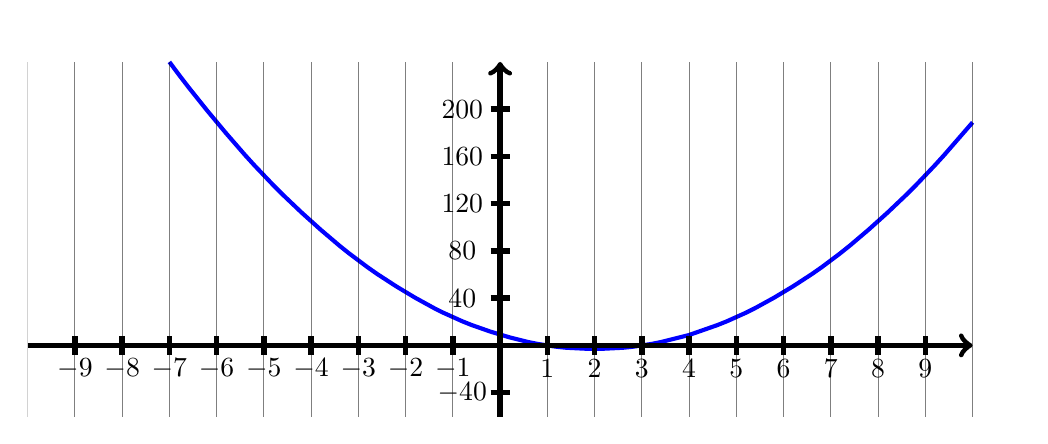
\begin{tikzpicture}[baseline,scale = 0.6]

        \tikzset{
          point/.style={
            thick,
            draw,
            cross out,
            inner sep=0pt,
            minimum width=5pt,
            minimum height=5pt,
          },
        }
        \clip (-10,-1.5) rectangle (11,6.725);
            
        \draw[color={blue},line width = 1.5] ;
        \draw[color={blue},line width = 1.5] ;
        \draw[color={blue},line width = 1.5] ;
        \draw[color={blue},line width = 1.5] ;
        \draw[color={blue},line width = 1.5] ;
        \draw[color={blue},line width = 1.5] ;
        \draw[color={blue},line width = 1.5] ;
        \draw[color={blue},line width = 1.5] ;
        \draw[color={blue},line width = 1.5] ;
        \draw[color={blue},line width = 1.5] ;
        \draw[color={blue},line width = 1.5] ;
        \draw[color={blue},line width = 1.5] ;
        \draw[color={blue},line width = 1.5] ;
        \draw[color={blue},line width = 1.5] ;
        \draw[color={blue},line width = 1.5] ;
        \draw[color={blue},line width = 1.5] (-7,6)--(-6.8,5.73)--(-6.6,5.47)--(-6.4,5.22)--(-6.2,4.97)--(-6,4.73)--(-5.8,4.49)--(-5.6,4.26)--(-5.4,4.03)--(-5.2,3.81)--(-5,3.6)--(-4.8,3.39)--(-4.6,3.19)--(-4.4,3)--(-4.2,2.81)--(-4,2.63)--(-3.8,2.45)--(-3.6,2.28)--(-3.4,2.11)--(-3.2,1.95)--(-3,1.8)--(-2.8,1.65)--(-2.6,1.51)--(-2.4,1.38)--(-2.2,1.25)--(-2,1.13)--(-1.8,1.01)--(-1.6,0.9)--(-1.4,0.79)--(-1.2,0.69)--(-1,0.6)--(-0.8,0.51)--(-0.6,0.43)--(-0.4,0.36)--(-0.2,0.29)--(0,0.23)--(0.2,0.17)--(0.4,0.12)--(0.6,0.07)--(0.8,0.03)--(1,0)--(1.2,-0.03)--(1.4,-0.05)--(1.6,-0.06)--(1.8,-0.07)--(2,-0.07)--(2.2,-0.07)--(2.4,-0.06)--(2.6,-0.05)--(2.8,-0.03)--(3,0)--(3.2,0.03)--(3.4,0.07)--(3.6,0.12)--(3.8,0.17)--(4,0.22)--(4.2,0.29)--(4.4,0.36)--(4.6,0.43)--(4.8,0.51)--(5,0.6)--(5.2,0.69)--(5.4,0.79)--(5.6,0.9)--(5.8,1.01)--(6,1.13)--(6.2,1.25)--(6.4,1.38)--(6.6,1.51)--(6.8,1.65)--(7,1.8)--(7.2,1.95)--(7.4,2.11)--(7.6,2.28)--(7.8,2.45)--(8,2.63)--(8.2,2.81)--(8.4,3)--(8.6,3.19)--(8.8,3.39)--(9,3.6)--(9.2,3.81)--(9.4,4.03)--(9.6,4.26)--(9.8,4.49)--(10,4.72);
        
        \draw[color ={black},line width = 2,->] (-10,0)--(10,0);
        \draw[color ={black},line width = 2,->] (0,-2)--(0,6);
        \draw[color ={black},opacity = 0.5] (1,-2)--(1,6);
        \draw[color ={black},opacity = 0.5] (2,-2)--(2,6);
        \draw[color ={black},opacity = 0.5] (3,-2)--(3,6);
        \draw[color ={black},opacity = 0.5] (4,-2)--(4,6);
        \draw[color ={black},opacity = 0.5] (5,-2)--(5,6);
        \draw[color ={black},opacity = 0.5] (6,-2)--(6,6);
        \draw[color ={black},opacity = 0.5] (7,-2)--(7,6);
        \draw[color ={black},opacity = 0.5] (8,-2)--(8,6);
        \draw[color ={black},opacity = 0.5] (9,-2)--(9,6);
        \draw[color ={black},opacity = 0.5] (10,-2)--(10,6);
        \draw[color ={black},opacity = 0.5] (-1,-2)--(-1,6);
        \draw[color ={black},opacity = 0.5] (-2,-2)--(-2,6);
        \draw[color ={black},opacity = 0.5] (-3,-2)--(-3,6);
        \draw[color ={black},opacity = 0.5] (-4,-2)--(-4,6);
        \draw[color ={black},opacity = 0.5] (-5,-2)--(-5,6);
        \draw[color ={black},opacity = 0.5] (-6,-2)--(-6,6);
        \draw[color ={black},opacity = 0.5] (-7,-2)--(-7,6);
        \draw[color ={black},opacity = 0.5] (-8,-2)--(-8,6);
        \draw[color ={black},opacity = 0.5] (-9,-2)--(-9,6);
        \draw[color ={black},opacity = 0.5] (-10,-2)--(-10,6);
        \draw[color ={black},line width = 2] (1,-0.2)--(1,0.2);
        \draw[color ={black},line width = 2] (2,-0.2)--(2,0.2);
        \draw[color ={black},line width = 2] (3,-0.2)--(3,0.2);
        \draw[color ={black},line width = 2] (4,-0.2)--(4,0.2);
        \draw[color ={black},line width = 2] (5,-0.2)--(5,0.2);
        \draw[color ={black},line width = 2] (6,-0.2)--(6,0.2);
        \draw[color ={black},line width = 2] (7,-0.2)--(7,0.2);
        \draw[color ={black},line width = 2] (8,-0.2)--(8,0.2);
        \draw[color ={black},line width = 2] (9,-0.2)--(9,0.2);
        \draw[color ={black},line width = 2] (-1,-0.2)--(-1,0.2);
        \draw[color ={black},line width = 2] (-2,-0.2)--(-2,0.2);
        \draw[color ={black},line width = 2] (-3,-0.2)--(-3,0.2);
        \draw[color ={black},line width = 2] (-4,-0.2)--(-4,0.2);
        \draw[color ={black},line width = 2] (-5,-0.2)--(-5,0.2);
        \draw[color ={black},line width = 2] (-6,-0.2)--(-6,0.2);
        \draw[color ={black},line width = 2] (-7,-0.2)--(-7,0.2);
        \draw[color ={black},line width = 2] (-8,-0.2)--(-8,0.2);
        \draw[color ={black},line width = 2] (-9,-0.2)--(-9,0.2);
        \draw[color ={black},line width = 2] (-0.2,1)--(0.2,1);
        \draw[color ={black},line width = 2] (-0.2,2)--(0.2,2);
        \draw[color ={black},line width = 2] (-0.2,3)--(0.2,3);
        \draw[color ={black},line width = 2] (-0.2,4)--(0.2,4);
        \draw[color ={black},line width = 2] (-0.2,5)--(0.2,5);
        \draw[color ={black},line width = 2] (-0.2,-1)--(0.2,-1);
        \draw [color={black},fill opacity = 1] (1,-0.5) node[anchor = center,scale=1] {$1$};
        \draw [color={black},fill opacity = 1] (2,-0.5) node[anchor = center,scale=1] {$2$};
        \draw [color={black},fill opacity = 1] (3,-0.5) node[anchor = center,scale=1] {$3$};
        \draw [color={black},fill opacity = 1] (4,-0.5) node[anchor = center,scale=1] {$4$};
        \draw [color={black},fill opacity = 1] (5,-0.5) node[anchor = center,scale=1] {$5$};
        \draw [color={black},fill opacity = 1] (6,-0.5) node[anchor = center,scale=1] {$6$};
        \draw [color={black},fill opacity = 1] (7,-0.5) node[anchor = center,scale=1] {$7$};
        \draw [color={black},fill opacity = 1] (8,-0.5) node[anchor = center,scale=1] {$8$};
        \draw [color={black},fill opacity = 1] (9,-0.5) node[anchor = center,scale=1] {$9$};
        \draw [color={black},fill opacity = 1] (-1,-0.5) node[anchor = center,scale=1] {$-1$};
        \draw [color={black},fill opacity = 1] (-2,-0.5) node[anchor = center,scale=1] {$-2$};
        \draw [color={black},fill opacity = 1] (-3,-0.5) node[anchor = center,scale=1] {$-3$};
        \draw [color={black},fill opacity = 1] (-4,-0.5) node[anchor = center,scale=1] {$-4$};
        \draw [color={black},fill opacity = 1] (-5,-0.5) node[anchor = center,scale=1] {$-5$};
        \draw [color={black},fill opacity = 1] (-6,-0.5) node[anchor = center,scale=1] {$-6$};
        \draw [color={black},fill opacity = 1] (-7,-0.5) node[anchor = center,scale=1] {$-7$};
        \draw [color={black},fill opacity = 1] (-8,-0.5) node[anchor = center,scale=1] {$-8$};
        \draw [color={black},fill opacity = 1] (-9,-0.5) node[anchor = center,scale=1] {$-9$};
        \draw [color={black},fill opacity = 1] (-0.8,1) node[anchor = center,scale=1] {$40$};
        \draw [color={black},fill opacity = 1] (-0.8,2) node[anchor = center,scale=1] {$80$};
        \draw [color={black},fill opacity = 1] (-0.8,3) node[anchor = center,scale=1] {$120$};
        \draw [color={black},fill opacity = 1] (-0.8,4) node[anchor = center,scale=1] {$160$};
        \draw [color={black},fill opacity = 1] (-0.8,5) node[anchor = center,scale=1] {$200$};
        \draw [color={black},fill opacity = 1] (-0.8,-1) node[anchor = center,scale=1] {$-40$};
    
    \end{tikzpicture}\\
    
\end{exercice}

\carreauxseyes{17.6}{13.6}

\end{document}